\documentclass[12pt,phd,times]{pkmthesis}
\usepackage{amsmath,epsfig,graphicx, subcaption,setspace,url,float}
\usepackage{pstricks,colortab,pifont}
\usepackage{lscape,multicol,multirow,longtable,subfigure}
\usepackage{cite, bm}                           % Due to this hyberref will not work for references (PKM on 07/07/08)
\usepackage{pdfpages}
\usepackage[english]{babel}
\usepackage[small,bf]{caption}              % Added on 26/08/08
%\usepackage{slashbox} 
\usepackage{csquotes}  
\usepackage{threeparttable}
\usepackage{longtable}
\restylefloat{table}
\usepackage{algorithm}
\usepackage{algorithmic}
%\usepackage{adjustbox}                    % Added on 24/10/08 (Senthil)
\setlength{\textfloatsep}{1cm}              % Spacing b/w  float and text (PKM 01/11/08)
%..........................................................................................................................................
\normalem                                   % Added on 01/07/08 to avoid underline in the references
\setlength{\abovecaptionskip}{8pt}          % Added on 08/07/08
\setlength{\belowcaptionskip}{8pt}          % Added on 08/07/08
%..........................................................................................................................................
\usepackage{hyperref}
\usepackage{extra_functions}
%\input{pagesetup_pkm_twoside.tex}           % Modified on 06/07/08, 10/07/08, 15/07/08
%\input{pagesetup_pkm_singleside.tex}       % For Single Sided Document 
\input{pagesetup_pkm_middleside.tex}       % Middle alignment 
\raggedbottom                               % o6/08/08  (Remove Unnecessary space b/w paragraphs)
%******************************************************************************************************************************************

\begin {document}
\setcounter{page}{1} \pagenumbering{roman}  % 03/07/08
\doublespacing                              % or use \baselineskip 12pt (12, 18 and 24)
%*************************************************** FRONT PAGES**********************************************
%\thispagestyle{empty}
%\pdfbookmark{Title}{Title}
%\begin{center}
\singlespacing
\vspace*{0.3cm}

{\large A report on}\par

\vspace{0.3cm}

{\fontsize{22pt}{28pt}\selectfont \textbf{Optimized Task Offloading for\\[0.25em] Healthcare IoT-Fog Systems}\par}

\vspace{0.35cm}

{\large submitted in partial fulfillment of the requirements for\\[0.2em]
\textbf{Summer Colloquium}\par}

\vspace{1.1cm}

{\large \textit{by}}\par
\vspace{0.15cm}
{\large \textbf{Tanneeru Vidath: 2023BCS-068}\par}

\vspace{0.9cm}

{\large Under the Supervision of}\par
\vspace{0.15cm}
{\large \textbf{Dr. Chittaranjan Swain}\par}
\vspace{0.2cm}
{\large Department of Computer Science and Engineering\par}

\vspace{0.8cm}


\includegraphics[width=3cm]{FrontPages/ABV_IIITM_logo.eps}\par

\vspace{0.6cm}

{\large ABV-INDIAN INSTITUTE OF INFORMATION TECHNOLOGY\\[0.15cm]
AND MANAGEMENT GWALIOR\\[0.15cm]
GWALIOR, INDIA\\[0.15cm]
AUGUST, 2026\par}

\end{center}





%\thispagestyle{empty}
%\clearpage

\thispagestyle{empty}
\pdfbookmark{Title}{Title}
\begin{center}
\singlespacing
\vspace*{0.3cm}

{\large A report on}\par

\vspace{0.3cm}

{\fontsize{22pt}{28pt}\selectfont \textbf{Optimized Task Offloading for\\[0.25em] Healthcare IoT-Fog Systems}\par}

\vspace{0.35cm}

{\large submitted in partial fulfillment of the requirements for\\[0.2em]
\textbf{Summer Colloquium}\par}

\vspace{1.1cm}

{\large \textit{by}}\par
\vspace{0.15cm}
{\large \textbf{Tanneeru Vidath: 2023BCS-068}\par}

\vspace{0.9cm}

{\large Under the Supervision of}\par
\vspace{0.15cm}
{\large \textbf{Dr. Chittaranjan Swain}\par}
\vspace{0.2cm}
{\large Department of Computer Science and Engineering\par}

\vspace{0.8cm}


\includegraphics[width=3cm]{FrontPages/ABV_IIITM_logo.eps}\par

\vspace{0.6cm}

{\large ABV-INDIAN INSTITUTE OF INFORMATION TECHNOLOGY\\[0.15cm]
AND MANAGEMENT GWALIOR\\[0.15cm]
GWALIOR, INDIA\\[0.15cm]
AUGUST, 2026\par}

\end{center}





\thispagestyle{empty}

\clearpage
\thispagestyle{empty}
\pdfbookmark{Dedication}{Dedication}
%\include{FrontPages/Dedication}

\thispagestyle{empty}
\pdfbookmark{Acknowledgement}{Acknowledgement}
\newpage
\begin{center}
{\large \bf DECLARATION}
\end{center}
I hereby certify that the work, which is being presented in the report, entitled \textbf{Optimized Task Offloading for Healthcare IoT-Fog Systems}, submitted to the institution, is an authentic record of my own work carried out during the period May 2026 to July 2026 under the supervision of Dr. Chittaranjan Swain. I also cited the references about the text(s)/figure(s)/table(s) from where they have been taken.
\vspace{0.6in} \\
Date: \hspace{3.2in} Signatures of the Candidate \\
\vspace{0.4in} \\
This is to certify that the above statement made by the candidates is correct to the best
 of my knowledge.
 \vspace{0.8in} \\
 Date: \hspace{3.2in} Signatures of the Supervisor \\


\clearpage
\thispagestyle{empty}
\pdfbookmark{Declaration}{Declaration}


\thispagestyle{empty}
\pdfbookmark{Acknowledgement}{Acknowledgement}
%\begin{acknowledgments}
\begin{center}
{\LARGE \bf Acknowledgements}
\end{center}
\noindent I would like to express my gratitude to Dr. Chittaranjan Swain for his guidance, patience, and advice throughout this project. His feedback helped shape the research direction and methodology.

\noindent I also thank the faculty of the Computer Science and Engineering Department for their encouragement and support. Additionally, I appreciate the research facilities provided by ABV-IIITM Gwalior.

\noindent Finally, I thank my peers and colleagues for their feedback, discussions, and support during this work.
\begin{flushright}
\textit{\textbf{Tanneeru Vidath}} \\
(2023BCS-068)
\end{flushright}

%\end{acknowledgments}




\thispagestyle{empty}
{\renewcommand{\baselinestretch}{1.5}
\begin{center}
    {\LARGE \bf Abstract}
\end{center}
{\em{\noindent In healthcare Internet of Things (IoT) systems, computational tasks generated by medical devices must be processed by nearby Fog Nodes (FNs) within strict deadlines. The existing Multi-Stage Deferred Acceptance Based Fair Task Offloading (M-DAFTO) algorithm treats all tasks in a single undifferentiated pool, uses only two urgency criteria, and employs a trivially consistent 2$\times$2 Analytic Hierarchy Process (AHP) matrix. Under high load, this causes critical surgical tasks to compete with routine checkups for the same resources, leading to unacceptable outages for life-critical operations.

This work adapts a severity-aware 2-Type Multi-Stage Deferred Acceptance (MSDA) algorithm that classifies tasks as Major (critical surgeries) or Minor (routine checkups) with separate quota constraints per fog node. The proposed approach extends the urgency function from two to four criteria by incorporating energy consumption and a severity multiplier, validated through a 4$\times$4 AHP matrix with full consistency checking (CR $\leq$ 0.1). Severity-weighted Min-Max normalisation is applied to both delay and energy, and separate preference lists are maintained for each task type. The 2-Type MSDA matching algorithm enforces three simultaneous constraints per fog node: Major quota limit, Minor quota limit, and total capacity limit.

The system was implemented in Java across 14 modular classes and evaluated against two baselines (Greedy Placement Method and M-DAFTO) over four task scales (250, 500, 1000, 2000) with 10 iterations each. The proposed method achieves 0\% critical-task outage under normal load (250--1000 tasks) and reduces overall outage by approximately 79\% and Major outage by approximately 89\% on average compared to the baseline, while maintaining comparable task satisfaction and delay metrics.

\vspace{0.4cm}
\noindent \textbf{\em Keywords:} Healthcare IoT, Fog Computing, Task Offloading, Matching Theory, 2-Type MSDA, Analytic Hierarchy Process (AHP), Resource Allocation.}}}
\thispagestyle{empty}
\clearpage


%..........................................................................................................................................
% For the fancy chapters (Don't remove these lines- 03/07/08)
\clearpage
\thispagestyle{empty}
\dominitoc
\dominilof
\dominilot
\fancyhf{} \fancyhead[LE]{\bfseries\small{\leftmark}}
\fancyhead[RO]{\bfseries\small{\rightmark}}
\fancyfoot[CE,CO]{\bfseries\thepage}
%..........................................................................................................................................
%TABLE OF CONTENTS
\renewcommand{\baselinestretch}{1}
\pdfbookmark[0]{Index}{index}
\pdfbookmark[1]{Contents}{toc}
\fancyhead[LE]{\bfseries\small{Contents}}
\fancyhead[RO]{\bfseries\small{Contents}}
\tableofcontents
\clearpage
%.........................................................................................................................................

%..........................................................................................................................................
% LIST OF ACRONYMS
\fancyhead[LE]{\bfseries\small{List of Acronyms}}
\fancyhead[RO]{\bfseries\small{List of Acronyms}}
\pdfbookmark[1]{List of Acronyms}{loa}
\addstarredchapter{List of Acronyms}
\chapter*{List of Acronyms}



\begin{longtable}{ll}

%A

AHP             & Analytic Hierarchy Process \\

%C

CI              & Consistency Index \\
CR              & Consistency Ratio \\

%D

DA              & Deferred Acceptance \\

%F

FN              & Fog Node \\

%G

GPM             & Greedy Placement Method \\

%I

IoT             & Internet of Things \\

%M

MCDM            & Multi-Criteria Decision Making \\
MSDA            & Multi-Stage Deferred Acceptance \\

%P

PL              & Preference List \\

%R

RI              & Random Index \\

%V

VRU             & Virtual Resource Unit \\

\end{longtable}

\clearpage
%..........................................................................................................................................
% % LIST OF SYMBOLS
% \fancyhead[LE]{\bfseries\small{List of Symbols}}
% \fancyhead[RO]{\bfseries\small{List of Symbols}}
% \pdfbookmark[1]{List of Symbols}{los}
% \addstarredchapter{List of Symbols}
% %\include{FrontPages/Symbols}
% \clearpage
%..........................................................................................................................................
\fancyhf{}
\fancyhead[LE]{\bfseries\small{\leftmark}}
\fancyhead[RO]{\bfseries\small{\rightmark}}
\fancyfoot[CE,CO]{\bfseries\thepage}
\setcounter{page}{1} \pagenumbering{arabic}
\renewcommand{\labelenumi}{(\roman{enumi})}   % Added on 09/08/2008
%*******************************************************************************************************************************************************************************************


%************************************************ BEGIN CHAPTERS **********************************************
\chapter{Introduction and Objectives}\label{chap:intro}
This chapter provides the context for this project and outlines the objectives to be achieved.

\section{Context}

The rapid growth of the Internet of Things (IoT) in healthcare has led to a proliferation of connected medical devices in smart hospital environments --- patient monitors, surgical equipment, diagnostic imaging systems, and environmental sensors \cite{swain2024mdafto}. These devices generate computational tasks that must be processed in real time. For instance, a surgery monitoring system cannot tolerate the 100+ millisecond latency of a distant cloud data centre; it requires single-digit millisecond response times.

Fog computing addresses this need by placing small edge servers --- called Fog Nodes (FNs) --- close to the data source, typically within the same building or campus \cite{chiti2018matching}. Compared to cloud computing, fog offers lower latency, reduced bandwidth consumption, higher reliability against internet outages, and stronger data privacy since sensitive patient information stays within the hospital network.

The core challenge addressed in this work is \textit{task offloading}: deciding which FN should process which task. Each IoT task has a strict deadline, each FN has limited capacity measured in Virtual Resource Units (VRUs), and network bandwidth is shared. Critically, not all tasks are equally important --- a major surgery matters far more than a routine checkup. If a task cannot be assigned to any FN, it results in an \textit{outage}. In healthcare, outages for critical operations are unacceptable.

This problem is fundamentally a multi-criteria matching problem: tasks have preferences over FNs (based on delay and energy), FNs have preferences over tasks (based on urgency), and both sides have constraints (deadlines, quotas). Standard load balancing optimises for a single metric and is insufficient. The Deferred Acceptance (DA) algorithm from matching theory \cite{gale1962college} provides a principled framework, and Multi-Stage Deferred Acceptance (MSDA) extends it with minimum-quota enforcement for fairness \cite{fragiadakis2016strategyproof}.

\section{Objectives}

The primary base paper, M-DAFTO \cite{swain2024mdafto}, proposes a Single-Type MSDA algorithm for IoT-fog task offloading. While effective, six key limitations can be identified:

\begin{itemize}
\item \textbf{Single-pool matching}: All tasks compete in one undifferentiated pool. A routine checkup competes for the same FN slots as a critical surgery, and under high load, critical tasks can be starved of resources.
\item \textbf{2-criteria urgency}: The urgency function uses only delay difference and preference count. Energy consumption --- a key concern in battery-powered IoT devices --- is completely ignored.
\item \textbf{No severity awareness}: There is no concept of task severity (Major vs Minor). The algorithm cannot prioritise critical healthcare operations over routine ones.
\item \textbf{Trivially consistent 2$\times$2 AHP}: With only 2 criteria, the Analytic Hierarchy Process (AHP) matrix is 2$\times$2 and always passes the consistency check (CR = 0 by definition).
\item \textbf{Delay-only normalisation}: Only delay is normalised via Min-Max scaling. Energy is neither normalised nor combined into the preference ordering.
\item \textbf{Single preference list per FN}: Each FN has one preference ranking over all tasks. There are no separate rankings for different task types.
\end{itemize}

The main objective is to adapt and implement a severity-aware 2-Type MSDA algorithm from \cite{oomori2026strategyproof} that overcomes all six limitations, while maintaining the theoretical guarantees of the original MSDA framework. Specifically, the project aims to:

\begin{enumerate}
\item Apply Major/Minor task classification with separate quota constraints based on the 2-Type framework of \cite{oomori2026strategyproof}.
\item Extend the urgency function from 2 to 4 criteria (adding energy and severity).
\item Implement a 4$\times$4 AHP matrix with genuine consistency validation.
\item Apply severity-weighted normalisation to both delay and energy.
\item Generate separate fog-side preference lists for Major and Minor tasks, as required by the 2-Type MSDA architecture \cite{oomori2026strategyproof}.
\item Evaluate the proposed method against two baselines across multiple load scales.
\end{enumerate}
%\clearpage
% \mbox{}
% \thispagestyle{empty}
% \newpage
%\fancychapter{Literature Review}
\chapter{Literature Review}\label{chap:L_surve}
% --- LITERATURE REVIEW ---
\noindent This chapter surveys the foundational theory and prior work relevant to this project, and identifies the gaps that motivate the proposed approach.

\section{Matching Theory Foundations}

The Deferred Acceptance (DA) algorithm, introduced by Gale and Shapley \cite{gale1962college}, solves the stable matching problem for two-sided markets. In DA, one side (proposers) makes offers to the other side (receivers). Each receiver tentatively accepts the best proposals up to its capacity and rejects the rest. Rejected proposers then propose to their next choice. This process repeats until no more proposals can be made. DA guarantees a stable matching --- no unmatched pair would both prefer each other over their current assignment.

Roth and Sotomayor \cite{roth1990twosided} provide the foundational theoretical treatment of two-sided matching, establishing key properties such as strategy-proofness for the proposing side and the lattice structure of stable matchings. Their work forms the basis for applying matching theory to resource allocation problems beyond the original marriage and college admissions settings.

Standard DA does not enforce minimum quotas --- some receivers may remain empty while others are overloaded. Kamada and Kojima \cite{kamada2015efficient} studied efficient matching under distributional constraints, showing that minimum-quota requirements can be incorporated while preserving desirable matching properties. Fragiadakis et al. \cite{fragiadakis2016strategyproof} formalised the Multi-Stage Deferred Acceptance (MSDA) algorithm with minimum quotas. MSDA runs DA in multiple stages: in early stages, tasks with the latest deadlines are removed from the pool and DA runs with maximum quotas; in the final stage, minimum quotas force remaining tasks onto receivers even if constraints are relaxed. This ensures every receiver gets at least its minimum quota.

The extension of MSDA to handle two types of agents with separate quota constraints was proposed by Oomori and Manabe \cite{oomori2026strategyproof}. Their 2-Type MSDA maintains four quota values per receiver: minimum and maximum quotas for all agents, and separate minimum and maximum quotas for one designated type (R-type). This theoretical framework is the basis for the matching algorithm adapted in this project.

\section{Task Offloading in IoT-Fog Systems}

Chiti et al. \cite{chiti2018matching} proposed a Matching-Based Task Offloading (MBTO) framework for IoT-fog systems, demonstrating that matching theory provides a principled approach to the task offloading problem. Their work showed that matching-based offloading outperforms greedy and random assignment strategies in terms of delay and resource utilisation.

Swain et al. \cite{swain2021leto} proposed LETO, a load-balanced task offloading strategy for IoT-fog systems that focused on distributing tasks fairly across fog nodes. LETO served as a direct predecessor to the M-DAFTO algorithm.

The M-DAFTO algorithm \cite{swain2024mdafto} extended the MSDA framework specifically for IoT-fog task offloading. M-DAFTO introduced a 2-criteria urgency function (based on delay difference and preference count), AHP-based weight generation, and multi-stage quota enforcement. M-DAFTO demonstrated improved fairness over prior approaches through its minimum-quota mechanism, which ensures that no fog node is left idle while others are overloaded.

\section{Gaps Identified}

Despite M-DAFTO's contributions, the following key gaps exist that limit its applicability to healthcare IoT:

\begin{enumerate}
\item \textbf{No task differentiation}: M-DAFTO treats all tasks in a single pool. In healthcare, a critical surgery and a routine checkup should not compete equally for resources.
\item \textbf{Limited urgency criteria}: Using only delay difference and preference count ignores energy consumption, which is important for battery-powered IoT devices.
\item \textbf{No severity awareness}: Without a severity concept, the algorithm cannot guarantee that critical tasks are assigned even under high load.
\item \textbf{Trivial AHP consistency}: The 2$\times$2 AHP matrix always has CR = 0, so no actual consistency validation occurs.
\item \textbf{Incomplete normalisation}: Only delay is normalised; energy values are neither scaled nor incorporated into the preference ordering.
\item \textbf{Single preference ranking}: Each fog node maintains only one preference list over all tasks, preventing type-specific prioritisation.
\end{enumerate}

These gaps motivate the adaptation of the 2-Type MSDA algorithm from \cite{oomori2026strategyproof}, combined with the proposed extensions: expanded urgency criteria, genuine AHP consistency checking, severity-weighted normalisation, and the mapping of Major/Minor healthcare task severity onto the R-type/S-type framework.
%\clearpage
% \mbox{}
% \thispagestyle{empty}
% \newpage

\chapter{System Model and Problem Formulation}\label{chap:system_model}
% --- SYSTEM MODEL AND PROBLEM FORMULATION ---

\noindent This chapter describes the system model, formulates the task offloading problem mathematically, and provides a recap of the baseline M-DAFTO algorithm.

\section{System Model}

This work considers a healthcare IoT-fog system consisting of IoT devices and Fog Nodes (FNs), building upon the architecture defined in the M-DAFTO base model \cite{swain2024mdafto}. The IoT devices generate computational tasks, and the FNs process them. Figure~\ref{fig:system_model} illustrates this architecture.

\begin{figure}[htbp]
\centering
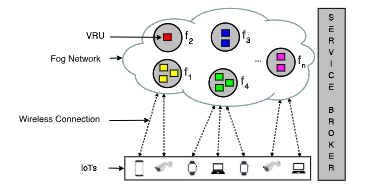
\includegraphics[width=0.85\textwidth]{Images/image1.png}
\caption{An IoT-Fog network comprising multiple IoT devices and FNs communicating over a wireless channel, adapted from \cite{swain2024mdafto}.}
\label{fig:system_model}
\end{figure}

\subsection{IoT Tasks}

Each IoT task $T_i$ (for $i = 1, 2, \ldots, M$) is characterised by:
\begin{itemize}
\item $\text{cpuDemanded}_i$: CPU demand in million cycles, drawn from $[210.0, 480.0]$ Mcycles.
\item $\text{inputSize}_i$: Input data size in KB, drawn from $[300.0, 600.0]$ KB.
\item $\text{outputSize}_i$: Output data size in KB, drawn from $[10.0, 20.0]$ KB.
\item $\text{deadline}_i$: Processing deadline in seconds, drawn from $[15.0, 22.0]$ s.
\item $\text{phase}_i$: Either ``Pre-Surgery'' or ``Post-Surgery'' (assigned randomly with equal probability).
\item $\text{severity}_i$: Either ``Major'' (critical operations) or ``Minor'' (routine tasks), assigned randomly with equal probability.
\end{itemize}

\subsection{Fog Nodes}

Each FN $F_j$ (for $j = 1, 2, \ldots, N$, where $N = 5$) is characterised by:
\begin{itemize}
\item $\text{totalCpuGHz}_j$: Total CPU capacity in GHz, drawn from $[6.0, 10.0]$ GHz.
\item $\text{numberOfVRUs}_j$: Number of Virtual Resource Units (VRUs), drawn from $[200, 500]$.
\item $\text{vruCapacity}_j = (\text{totalCpuGHz}_j \times 1000) / \text{numberOfVRUs}_j$ (Mcycles/s per VRU).
\end{itemize}

A VRU is a logical unit of compute capacity. A fog node with 400 VRUs can theoretically handle 400 concurrent tasks. The maximum quota of a fog node equals its number of VRUs.

\section{Problem Formulation}

\subsection{Offloading Delay}

For task $T_i$ offloaded to fog node $F_j$, the offloading delay is:
\begin{equation}
\text{delay}_{ij} = \text{txTime}_{ij} + \text{execTime}_{ij} + \text{rxTime}_{ij}
\end{equation}
where:
\begin{align}
\text{txTime}_{ij} &= \frac{\text{inputSize}_i}{\text{UPLINK\_DATA\_RATE}} \\
\text{execTime}_{ij} &= \frac{\text{cpuDemanded}_i}{\text{vruCapacity}_j} \\
\text{rxTime}_{ij} &= \frac{\text{outputSize}_i}{\text{DOWNLINK\_DATA\_RATE}}
\end{align}

The uplink and downlink data rates are both 2500.0 KB/s (derived from 20 MHz bandwidth).

\subsection{Energy Consumption}

The energy consumed when task $T_i$ is offloaded to fog node $F_j$ is:
\begin{equation}
\text{energy}_{ij} = (P_{\text{tx}} \times \text{txTime}_{ij}) + (P_{\text{exec}} \times \text{execTime}_{ij}) + (P_{\text{rx}} \times \text{rxTime}_{ij})
\end{equation}
where $P_{\text{tx}} = 0.5$ W (transmission power), $P_{\text{exec}} = 1.0$ W (execution power), and $P_{\text{rx}} = 0.5$ W (receiving power).

\subsection{Assignment Constraints}

A valid task assignment must satisfy:
\begin{itemize}
\item Each task is assigned to at most one fog node.
\item The number of tasks assigned to fog node $F_j$ must not exceed its maximum quota $q_j = \text{numberOfVRUs}_j$.
\item The number of tasks assigned to $F_j$ must meet its minimum quota $p_j$ (for fairness).
\item An unassigned task constitutes an \textit{outage}.
\end{itemize}

\section{Baseline M-DAFTO Recap}

The M-DAFTO algorithm \cite{swain2024mdafto} uses a Single-Type MSDA (Algorithm 9 from \cite{fragiadakis2016strategyproof}) with the following characteristics:

\subsection{2-Criteria Urgency Function}

For task $T_i$ at fog node $F_j$:
\begin{equation}
U(T_i, F_j) = w_1 \times \frac{1}{\text{deadline}_i - \text{delay}_{ij}} + w_2 \times \frac{1}{\text{pref}(T_i)}
\end{equation}
where $\text{pref}(T_i)$ is the number of fog nodes where $\text{delay}_{ij} \leq \text{deadline}_i$ (if 0, set to 1.0 to avoid division by zero), and $w_1, w_2$ are weights generated by a 2$\times$2 AHP matrix.

\subsection{2$\times$2 AHP Weight Generation}

M-DAFTO generates weights using a 2$\times$2 pairwise comparison matrix. With only 2 criteria, the matrix always passes the consistency check (CR = 0 by definition), providing no actual validation.

\subsection{Quota Determination}

Minimum quotas are computed proportionally based on VRU capacity relative to the most efficient node. For each fog node $F_j$:
\begin{equation}
p_j = \min\left(\left\lfloor \frac{\text{vruCapacity}_j}{\lambda_{\max}} \times l_{\max} \right\rfloor, \; \text{numberOfVRUs}_j\right)
\end{equation}
where $\lambda_{\max}$ is the maximum VRU capacity across all fog nodes, and $l_{\max} = \min(h_{\max}, \lfloor |T| / |F| \rfloor)$ with $h_{\max}$ being the number of VRUs of the most efficient node. Maximum quotas equal the number of VRUs.

\subsection{Time Complexity}

M-DAFTO achieves a time complexity of $O(m \cdot n)$ per DA round, where $m$ is the number of tasks and $n$ is the number of fog nodes \cite{swain2024mdafto}.
%\clearpage
%\mbox{}
%\thispagestyle{empty}
%\newpage

\chapter{Proposed Methodology}\label{chap:methodology}
% --- PROPOSED 2-TYPE MSDA METHODOLOGY ---

\noindent This chapter presents the proposed methodology in detail. The system architecture involves a complete pipeline from task generation and severity classification, through urgency scoring using an extended Analytic Hierarchy Process (AHP), to the final task assignment using an adapted 2-Type Multi-Stage Deferred Acceptance (MSDA) algorithm.

\section{Overview of the Proposed Pipeline}

The proposed system replaces the baseline M-DAFTO single-pool approach with a severity-aware matching pipeline. The pipeline operates in sequential stages to ensure that critical healthcare tasks are prioritised without entirely starving routine tasks. First, tasks are generated and classified by severity. Second, delay and energy costs are calculated and normalised. Third, a 4-criteria AHP model generates dynamic weights to compute an urgency score for each task-node pair. Finally, the adapted 2-Type MSDA algorithm uses these urgency scores to form preference lists and execute the matching process.

\section{Severity-Aware Task Classification and Quotas}

Unlike the baseline M-DAFTO algorithm which treats all tasks equally, the proposed system categorises tasks into two distinct classes based on the framework introduced by Oomori and Manabe \cite{oomori2026strategyproof}:
\begin{itemize}
\item \textbf{Major Tasks (R-type):} Critical healthcare operations, such as surgical robotic control or emergency patient monitoring.
\item \textbf{Minor Tasks (S-type):} Routine healthcare operations, such as regular data logging or non-urgent checkups.
\end{itemize}

To ensure Major tasks are never starved of computational resources during high-load scenarios, the system enforces a strict quota structure on every fog node. 
Figure~\ref{fig:quota_structure} illustrates this quota tracking mechanism. Each fog node maintains four quota values:
\begin{itemize}
\item $p_c$: minimum quota for all tasks
\item $q_c$: maximum quota for all tasks (= numberOfVRUs)
\item $pr_c$: minimum guaranteed quota for Major tasks
\item $qr_c$: maximum allowed quota for Major tasks
\end{itemize}

\begin{figure}[htbp]
\centering
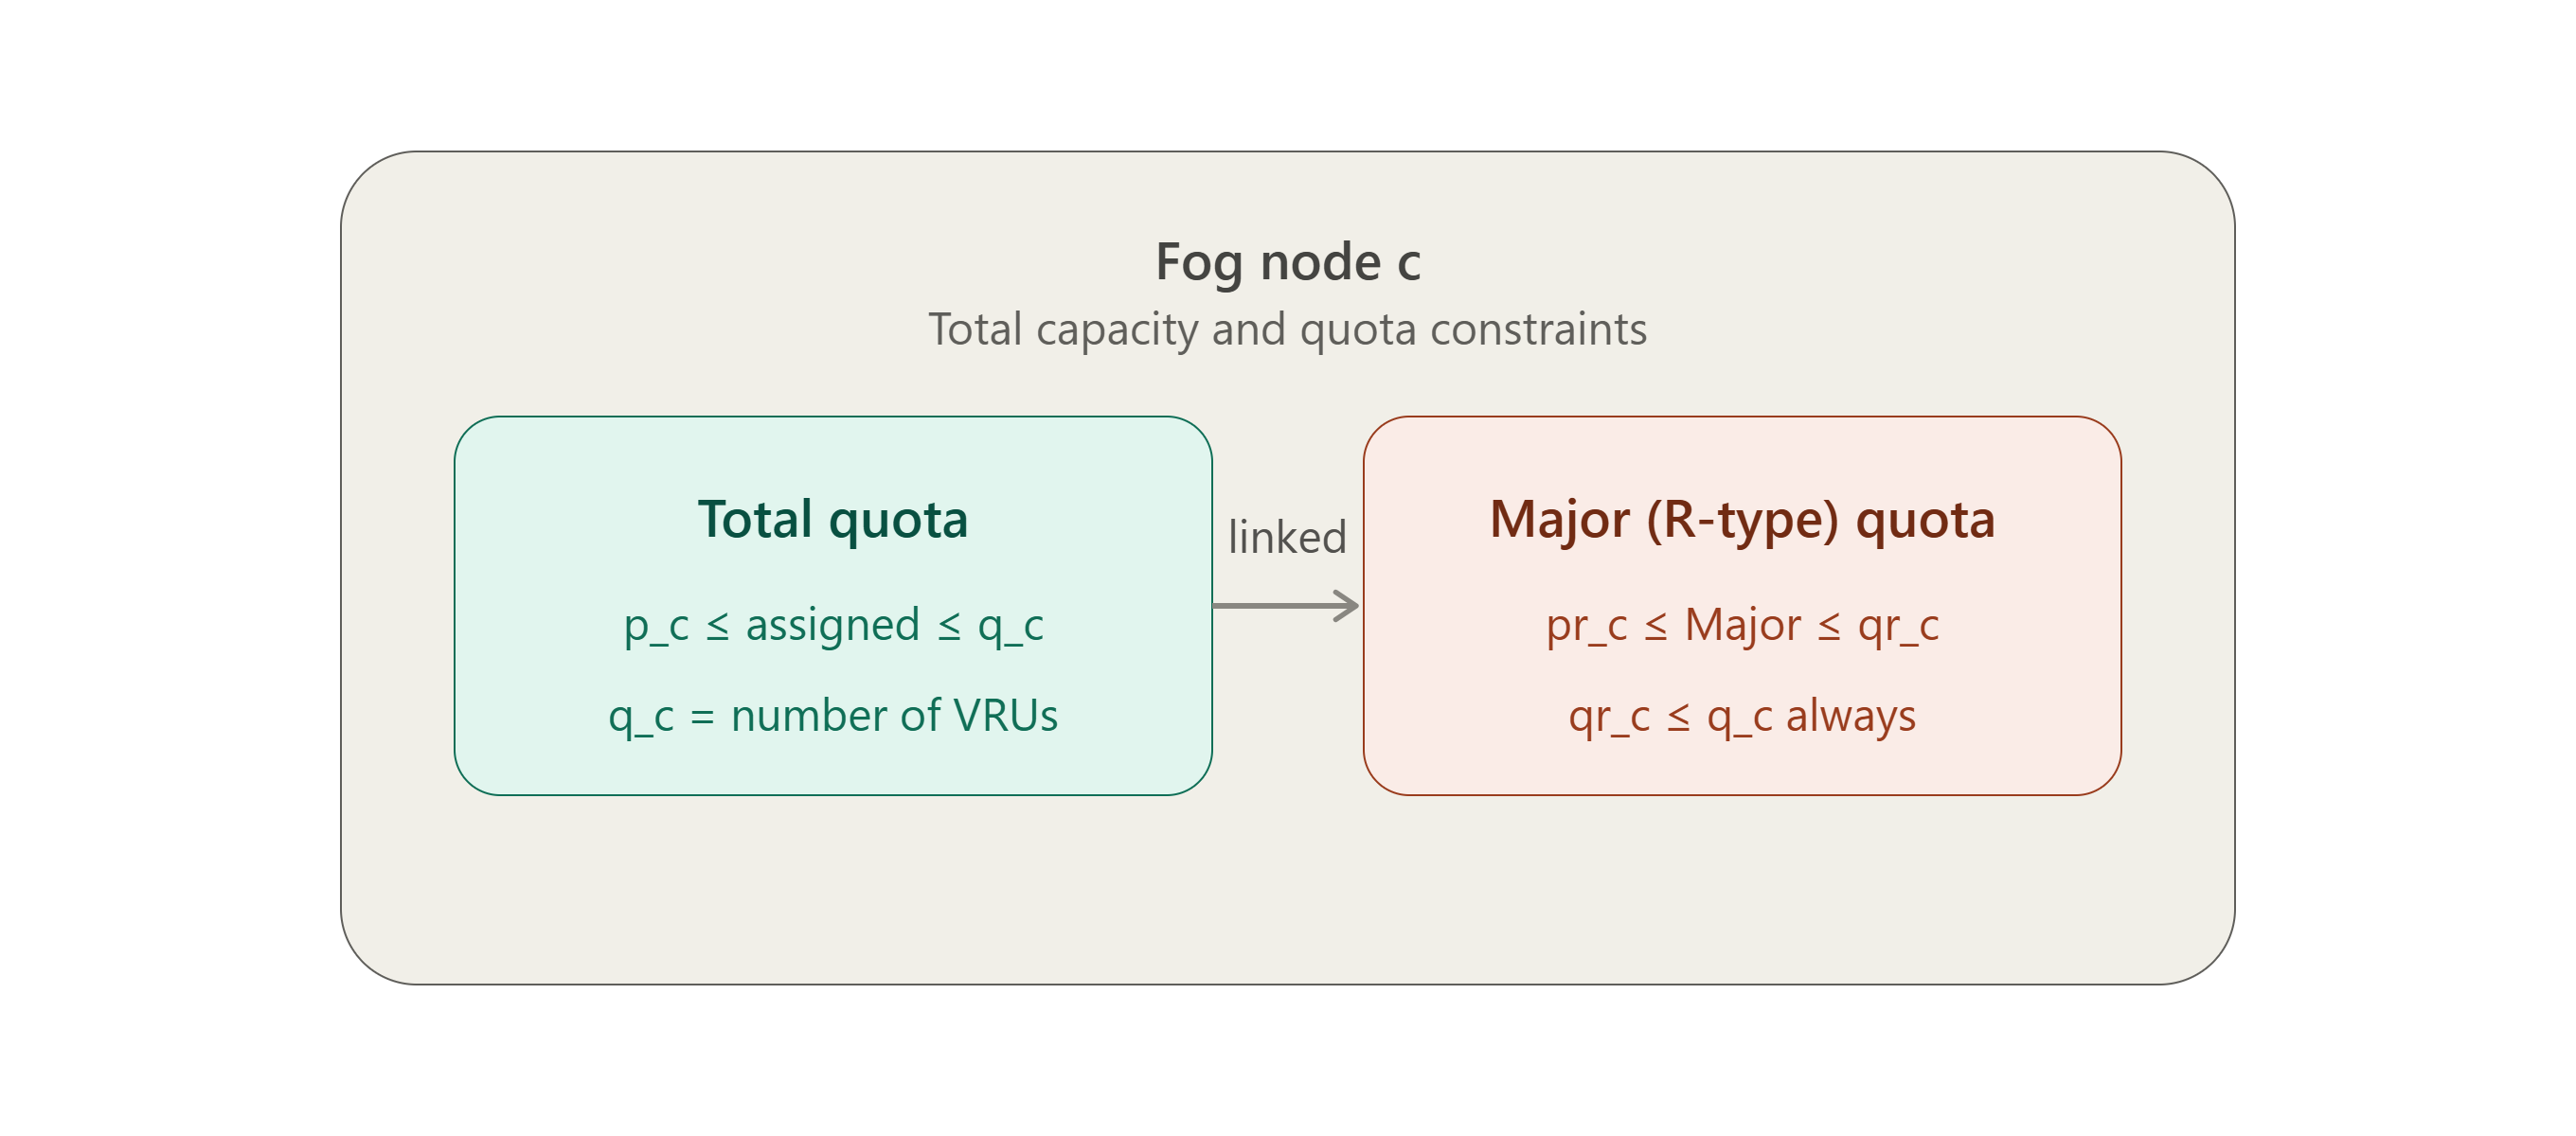
\includegraphics[width=0.85\textwidth]{Images/fog_node_quota_structure.png}
\caption{Fog node quota structure showing separate quota tracking for Major (R-type) and Minor (S-type) tasks, adapted from \cite{oomori2026strategyproof}.}
\label{fig:quota_structure}
\end{figure}

\section{The Severity-Aware 4-Criteria Urgency Model}

Before tasks can be matched to fog nodes, they must rank the fog nodes based on urgency. The baseline M-DAFTO model relies on a simple 2-criteria urgency function (delay and preference count). The proposed system introduces a novel 4-criteria model that incorporates both energy consumption and explicit severity weighting.

\subsection{Severity-Weighted Normalisation}
Delay (measured in seconds) and Energy (measured in Joules) operate on vastly different scales. A severity-weighted Min-Max normalisation is introduced to align these metrics:
\begin{equation}
\text{weight} = \begin{cases} 0.5 & \text{if severity} = \text{``Minor''} \\ 1.0 & \text{if severity} = \text{``Major''} \end{cases}
\end{equation}
\begin{align}
nd_{ij} &= \frac{\text{delay}_{ij} - \text{minDelay}}{\text{maxDelay} - \text{minDelay}} \times \text{weight} \\
ne_{ij} &= \frac{\text{energy}_{ij} - \text{minEnergy}}{\text{maxEnergy} - \text{minEnergy}} \times \text{weight}
\end{align}

\subsection{Severity Score}
To actively push Major tasks higher in the preference rankings, a severity multiplier $\gamma(T_i)$ is dynamically calculated:
\begin{equation}
\gamma(T_i) = 1 + c_i \times 0.5
\end{equation}
where $c_i = 1$ for Major tasks and $c_i = 0$ for Minor tasks. This forces $\gamma = 1.5$ for critical tasks and $\gamma = 1.0$ for routine tasks.

\subsection{4-Criteria Urgency Function and AHP}
The final urgency function $U(T_i, F_j)$ for a task $T_i$ on fog node $F_j$ is computed as:
\begin{equation}
U(T_i, F_j) = w_1 \frac{1}{\Delta d} + w_2 \frac{1}{\text{pref}(T_i)} + w_3 \frac{1}{\text{energy}_{ij}} + w_4 \gamma(T_i)
\end{equation}
where $\Delta d = \text{deadline}_i - \text{delay}_{ij}$.

The weights $w_1 \ldots w_4$ are generated using a 4$\times$4 Analytic Hierarchy Process (AHP) matrix. The weight generation process follows three rigorous steps \cite{saaty1980ahp}:

\textbf{1. Pairwise Matrix Construction (PMC):} Four random values $v[1..4]$ are drawn from $[1.0, 9.0]$. The pairwise comparison matrix $P$ is built where $P_{xy} = \text{getSaatyScale}(v_x / v_y)$ for $x < y$, with $P_{yx} = 1/P_{xy}$ and $P_{xx} = 1.0$.

\textbf{2. Column Weight Determination (CWD):} The matrix $P$ is column-normalised to produce $\bar{P}$, and the rows of $\bar{P}$ are averaged to obtain the final weights $W = [w_1, w_2, w_3, w_4]^T$.

\textbf{3. Consistency Check (CC):} 
Unlike the baseline's 2$\times$2 matrix which is trivially consistent (CR = 0 always), this 4$\times$4 matrix requires genuine consistency validation. The maximum eigenvalue $\lambda_{\max}$ is computed:
\begin{align}
\lambda_{\max} &= \text{average}\left(\frac{\text{rowSum}(P \cdot W)}{W_x}\right) \\
CI &= \frac{\lambda_{\max} - n}{n - 1}, \quad RI = 0.90 \text{ (for } n=4\text{)} \\
CR &= \frac{CI}{RI}
\end{align}
The generated weights are only accepted if $CR \leq 0.1$. Otherwise, the matrix is regenerated.

\section{The 2-Type MSDA Matching Engine}

Before executing the matching algorithm, the system must generate preference and precedence lists to dictate the order of matching, as structurally required by the MSDA framework.

\subsection{Preference and Precedence Lists}
\begin{itemize}
\item \textbf{Task Preference Lists:} During the deferred acceptance process, each task $T_i$ must propose to fog nodes in its order of preference. A task's preference list (\texttt{preferredFogIndices}) is constructed by sorting all available fog nodes in ascending order of their combined normalised cost, \texttt{normSum} ($nd_{ij} + ne_{ij}$). This ensures that tasks always propose to the most delay-and-energy efficient fog nodes first.
\item \textbf{Fog Node Preference Lists:} Each fog node $F_j$ evaluates all tasks using the 4-criteria urgency function $U(T_i, F_j)$ to determine its own preferences. It generates three separate sorted rankings: one for all tasks, one strictly for Major tasks, and one strictly for Minor tasks.
\item \textbf{Task Precedence Lists:} To determine which tasks propose first during the deferred acceptance rounds, tasks are placed into precedence lists sorted strictly by their tightest deadlines. Separate precedence lists are maintained for Major and Minor tasks.
\end{itemize}

These lists are then fed into the adapted 2-Type MSDA algorithm.

\begin{figure}[htbp]
\centering
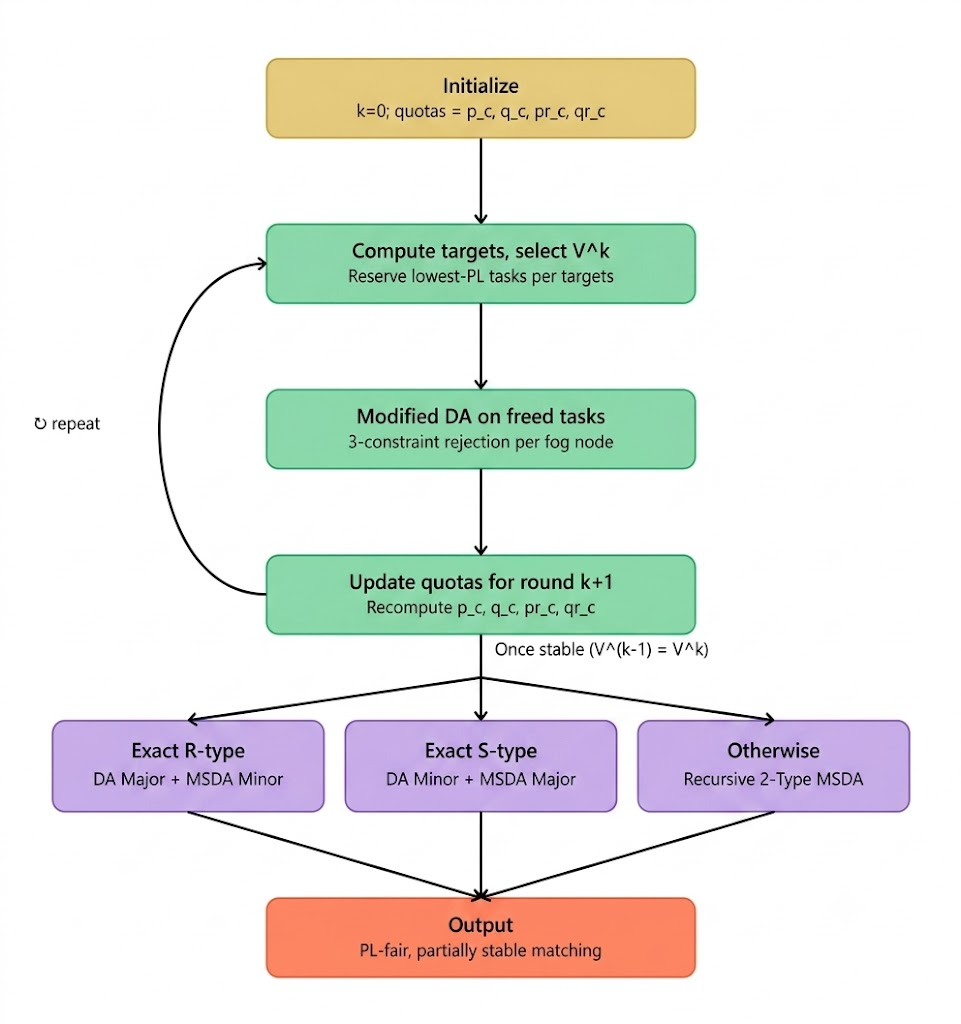
\includegraphics[width=0.95\textwidth]{Images/two_type_msda_algorithm_flow.png}
\caption{Flowchart of the adapted 2-Type MSDA matching engine, adapted from \cite{oomori2026strategyproof}.}
\label{fig:algorithm_flow}
\end{figure}

The matching engine utilises a Modified Deferred Acceptance (Modified DA) sub-routine. As shown in Algorithm \ref{alg:modified_da}, this routine simultaneously enforces the strict Major and Minor capacity constraints defined by the fog node quotas.

\begin{algorithm}[htbp]
\caption{Modified Deferred Acceptance (Fog Node Receiver Logic)}
\label{alg:modified_da}
\begin{algorithmic}[1]
\REQUIRE New proposal from task $T_i$ to Fog Node $F_j$
\vspace{1.5mm}
\STATE \textbf{Action:} $F_j$ tentatively accepts $T_i$.
\STATE \textbf{Constraint Checks:}
\WHILE{$F_j$ violates any constraint}
    \IF{Accepted Major tasks $> qr_c$}
        \STATE Reject the lowest-ranked \textbf{Major} task currently held by $F_j$.
    \ENDIF
    \IF{Accepted Minor tasks $> q_c - pr_c$}
        \STATE Reject the lowest-ranked \textbf{Minor} task currently held by $F_j$.
    \ENDIF
    \IF{Total accepted tasks $> q_c$}
        \STATE Find lowest-ranked Major task ($M_{worst}$) and Minor task ($m_{worst}$).
        \STATE Reject whichever is ranked lower overall between $M_{worst}$ and $m_{worst}$.
    \ENDIF
\ENDWHILE
\end{algorithmic}
\end{algorithm}

\newpage
The outer loop of the matching engine handles the multi-stage quota enforcement, mathematically defined in Algorithm \ref{alg:two_type_msda}. To formally track the assignment process across multiple iterations, the following notations are introduced:
\begin{itemize}
\item $k$: The current iteration index of the multi-stage algorithm.
\item $V^k$: The set of active tasks making proposals during iteration $k$.
\item $vs^k, vr^k, vt^k$: The aggregated target minimum quotas remaining across all fog nodes for Minor tasks, Major tasks, and all tasks combined, respectively, at iteration $k$.
\item $\mu^k$: The tentative matching outcome resulting from the Modified DA execution in iteration $k$.
\item $p_j^k, q_j^k, pr_j^k, qr_j^k$: The dynamically updated remaining quotas for fog node $F_j$ at iteration $k$.
\end{itemize}

By iteratively tightening the active set of tasks $V^k$ based on the remaining aggregate quotas, the engine guarantees that Major tasks secure their minimum quotas $pr_j$ without exceeding their strict ceilings $qr_j$. Once targets are met, the algorithm recursively branches to execute standard DA or MSDA for the remaining subgroups.

\begin{algorithm}[htbp]
\caption{Adapted 2-Type MSDA Algorithm}
\label{alg:two_type_msda}
\begin{algorithmic}[1]
\STATE Set $k = 0$, $V^0 = T$, $p_j^1 = p_c$, $q_j^1 = q_c$, $pr_j^1 = pr_c$, and $qr_j^1 = qr_c$ for all $F_j \in F$.
\REPEAT
    \STATE $k = k + 1$
    \STATE Let $vs^k = \sum_{F_j \in F} \max(0, p_j^k - qr_j^k)$, $vr^k = \sum_{F_j \in F} pr_j^k$, and $vt^k = \sum_{F_j \in F} p_j^k$.
    \STATE Set $V^k$ be the minimum set of tasks with the lowest priority according to $\succ$ which satisfies $|V^k| \geq vt^k$, $|V^k \cap T_{Minor}| \geq vs^k$, and $|V^k \cap T_{Major}| \geq vr^k$.
    \IF{$V^{k-1} \setminus V^k \neq \emptyset$}
        \STATE Execute Modified DA (Algorithm \ref{alg:modified_da}) on the tasks in $V^{k-1} \setminus V^k$. Let $\mu^k$ be the matching in this round.
        \FOR{each $F_j \in F$}
            \STATE $q_j^{k+1} = q_j^k - |\mu^k(F_j)|$,
            \STATE $qr_j^{k+1} = \min(qr_j^k - |\mu^k(F_j) \cap T_{Major}|, q_j^{k+1})$,
            \STATE $pr_j^{k+1} = \max(0, pr_j^k - |\mu^k(F_j) \cap T_{Major}|)$, and
            \STATE $p_j^{k+1} = \max(0, p_j^k - |\mu^k(F_j) \cap T_{Minor}| - \max(pr_j^k, |\mu^k(F_j) \cap T_{Major}|)) + pr_j^{k+1}$.
        \ENDFOR
    \ELSE
        \STATE Let $F' (\subseteq F)$ be the set of fog nodes which satisfies $p_j^k > 0$.
        \IF{$|V^k \cap T_{Major}| == vr^k$}
            \STATE Execute Standard DA on $V^k \cap T_{Major}$ and every fog node $F_j \in F'$ with $pr_j = qr_j = qr_j^k$. (For other $F_{j'} \notin F'$, set $pr_{j'} = qr_{j'} = 0$.)
            \STATE Execute Single-Type MSDA on $V^k \cap T_{Minor}$ with $p_j = p_j^k - pr_j^k$ and $q_j = q_j^k - pr_j^k$ for $F_j \in F'$ and $p_{j'} = 0$, $q_{j'} = q_{j'}^k$ for $F_{j'} \notin F'$.
            \STATE \textbf{exit} /* end of the algorithm */
        \ELSIF{$|V^k \cap T_{Minor}| == vs^k$}
            \STATE Execute Standard DA on $V^k \cap T_{Minor}$ and every fog node $F_j \in F'$ with $p_j = q_j = \max(p_j^k - qr_j^k, 0)$. (For other $F_{j'} \notin F'$, set $p_{j'} = q_{j'} = 0$.)
            \STATE Execute Single-Type MSDA on $V^k \cap T_{Major}$ with $pr_j = pr_j^k$ and $qr_j = qr_j^k$ for $F_j \in F'$ and $pr_{j'} = 0$, $qr_{j'} = qr_{j'}^k$ for $F_{j'} \notin F'$.
            \STATE \textbf{exit} /* end of the algorithm */
        \ELSE
            \STATE /* $|V^k \cap T_{Major}| > vr^k$ and $|V^k| == vt^k$ */
            \STATE Execute Adapted 2-Type MSDA on tasks in $V^k$ and every fog node $F_j \in F'$ with $pr_j = p_j = pr_j^k$, $qr_j = \min(qr_j^k, p_j^k)$, and $q_j = p_j^k$. (For other $F_{j'} \notin F'$, set $p_{j'} = q_{j'} = pr_{j'} = qr_{j'} = 0$.)
            \STATE \textbf{exit} /* end of the algorithm */
        \ENDIF
    \ENDIF
\UNTIL{forever}
\end{algorithmic}
\end{algorithm}

\section{Algorithmic Complexity}
A single Deferred Acceptance round has a complexity of $O(T \times F)$ where $T$ is the number of tasks and $F$ is the number of fog nodes. The MSDA stages are inherently bounded by $T$ because each stage successfully matches at least one task or exhausts a quota. Therefore, the worst-case overall complexity is $O(T^2 \times F)$. In practice, convergence is significantly faster because the tight quota constraints limit the number of required matching stages. The Modified DA adds a negligible constant-factor overhead for enforcing the three simultaneous constraints.

%\clearpage
%\mbox{}
%\thispagestyle{empty}
%\newpage

\chapter{Implementation and Experimental Setup}\label{chap:implementation}
% --- IMPLEMENTATION AND EXPERIMENTAL SETUP ---

\noindent This chapter describes the Java implementation architecture and the experimental setup used to evaluate the proposed algorithm.

\section{Java Architecture}

The entire system was implemented in Java (JDK 8+) using a modular pipeline architecture across 14 classes and approximately 2,500 lines of code. Each phase of computation is a separate, self-contained class, and data flows through the pipeline via a central data transfer object (SimulationData). Figure~\ref{fig:pipeline_arch} shows the overall architecture.

\begin{figure}[htbp]
\centering
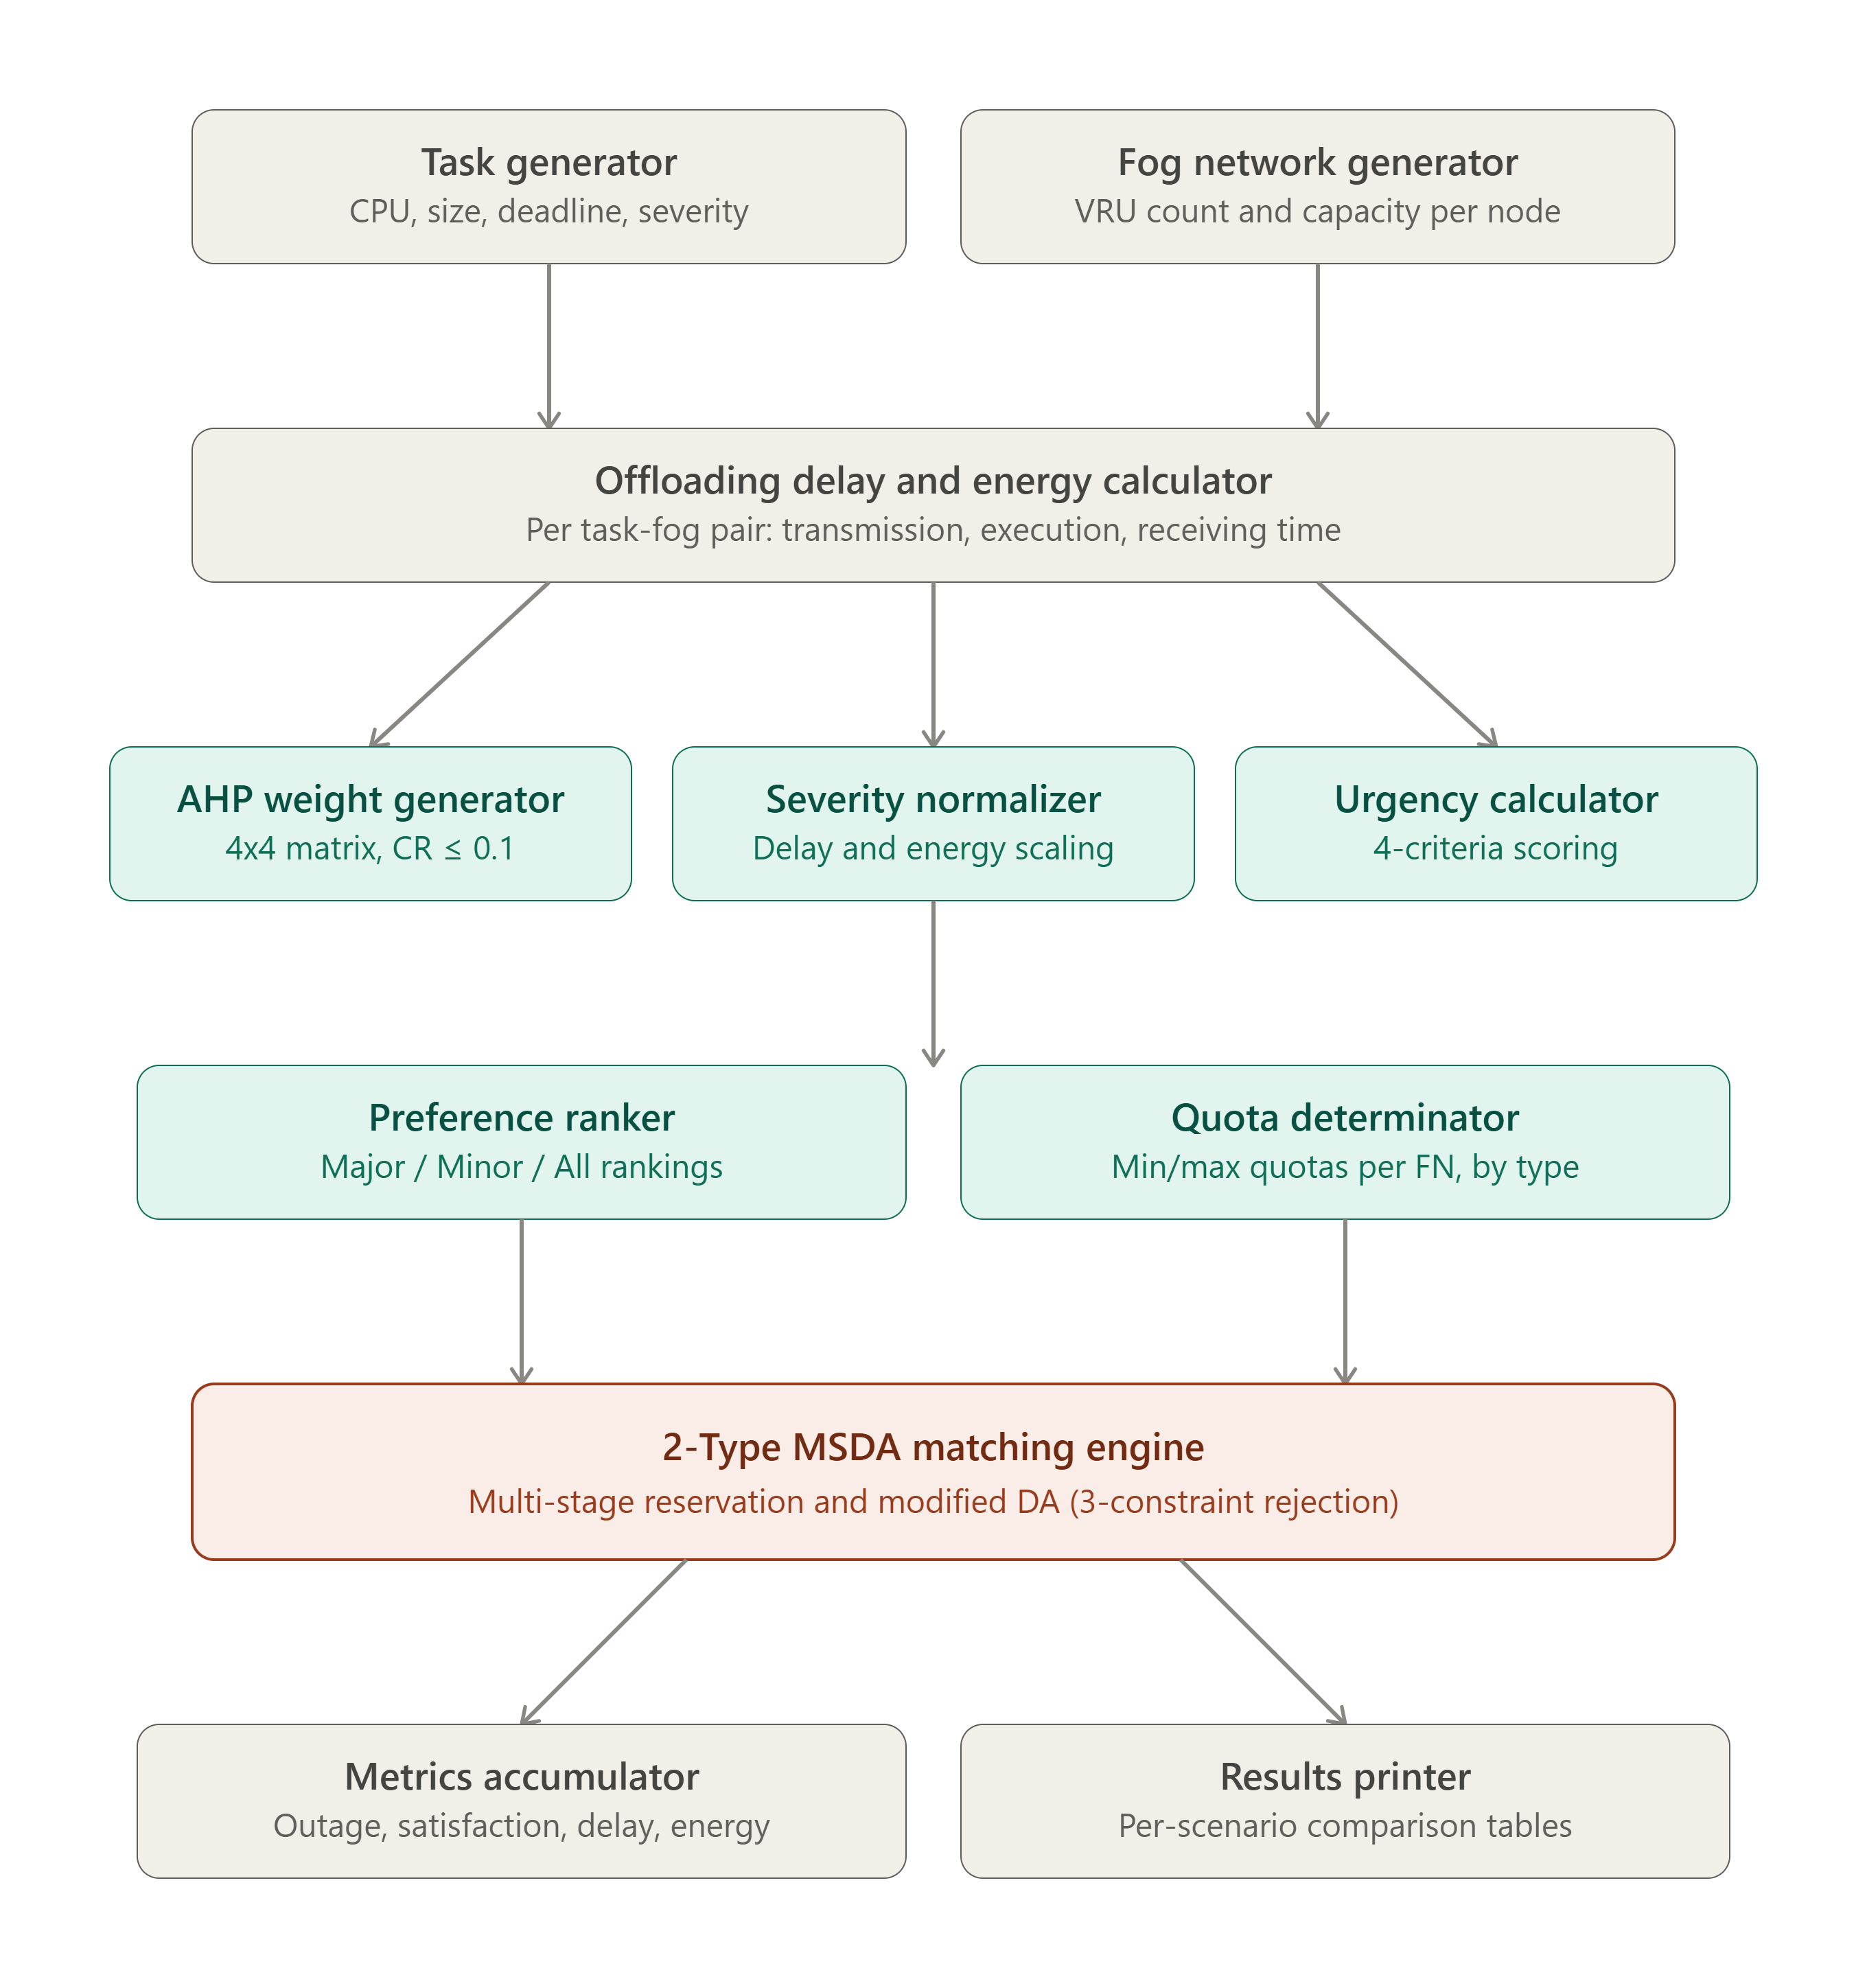
\includegraphics[width=0.95\textwidth]{Images/proposed_2type_msda_pipeline_architecture.png}
\caption{Modular pipeline architecture of the Java implementation showing the 14 classes and data flow.}
\label{fig:pipeline_arch}
\end{figure}

\begin{table}[htbp]
\centering
\begin{tabular}{|l|l|l|}
\hline
\textbf{Category} & \textbf{File} & \textbf{Responsibility} \\
\hline
Orchestrator & Main.java & Entry point; runs full pipeline across scenarios \\
\hline
\multirow{4}{*}{Data Models} & Task.java & Task attributes and per-fog metric arrays \\
 & FogNetwork.java & FN attributes, capacity, and quota fields \\
 & SimulationData.java & DTO bundling all computed arrays \\
 & SimulationConfig.java & Central constants and parameter ranges \\
\hline
\multirow{2}{*}{Generators} & TaskGenerator.java & Random IoT task generation \\
 & FogNetworkGenerator.java & Random fog node generation \\
\hline
\multirow{4}{*}{Calculators} & OffloadingCalculator.java & Delay and energy computation \\
 & Normalizer.java & Min-Max + severity-weight normalisation \\
 & UrgencyCalculator.java & Multi-criteria urgency scoring \\
 & QuotaDeterminator.java & Min/max quota computation \\
\hline
\multirow{2}{*}{Ranking \& Matching} & WeightGenerator.java & AHP 4$\times$4 with CR $\leq$ 0.1 \\
 & PreferenceRanker.java & Fog-side rankings and precedence lists \\
\hline
Matching & MSDAlgorithm.java & Single-Type MSDA, 2-Type MSDA, GPM \\
\hline
\multirow{2}{*}{Output} & SimulationPrinter.java & Results, tables, and utilisation bars \\
 & SimulationMetrics.java & Accumulator for averaging across iterations \\
\hline
\end{tabular}
\caption{File structure and responsibilities of the 14-class Java implementation.}
\label{tab:file_structure}
\end{table}

A critical design decision was the use of deep copy to ensure data independence between algorithm pipelines. All three algorithms (GPM, Baseline, Proposed) start from identical raw data (same fog nodes, same tasks, same delays, same energies). The deep copy creates independent copies so each algorithm modifies its own data without contaminating the others, guaranteeing a fair apples-to-apples comparison.

\section{Experimental Setup}

\subsection{Algorithms Compared}

Three algorithms are evaluated and compared:
\begin{enumerate}
\item \textbf{Greedy Placement Method (GPM)}: Assigns tasks greedily to fog nodes sorted by capacity, with no fairness or urgency considerations. Provides a lower-bound comparison.
\item \textbf{Baseline (M-DAFTO)}: Single-Type MSDA with 2-criteria urgency, 2$\times$2 AHP, and delay-only normalisation \cite{swain2024mdafto}.
\item \textbf{Proposed System (Adapted 2-Type MSDA)}: Severity-aware 2-Type MSDA with 4-criteria urgency, 4$\times$4 AHP, severity-weighted normalisation, and separate Major/Minor quota tracking.
\end{enumerate}

\subsection{Simulation Parameters}

\begin{table}[htbp]
\centering
\begin{tabular}{|l|l|}
\hline
\textbf{Parameter} & \textbf{Range / Value} \\
\hline
Number of tasks & 250, 500, 1000, 2000 (per scenario) \\
Number of fog nodes & 5 \\
CPU demand & [210.0, 480.0] Mcycles \\
Input size & [300.0, 600.0] KB \\
Output size & [10.0, 20.0] KB \\
Deadline & [15.0, 22.0] seconds \\
Fog CPU capacity & [6.0, 10.0] GHz \\
Fog VRU count & [200, 500] \\
Phase & ``Pre-Surgery'' / ``Post-Surgery'' \\
Severity & ``Minor'' / ``Major'' (50/50) \\
Uplink data rate & 2500 KB/s (20 MHz) \\
Downlink data rate & 2500 KB/s (20 MHz) \\
Transmission power & 0.5 W \\
Execution power & 1.0 W \\
Receiving power & 0.5 W \\
\hline
\end{tabular}
\caption{Simulation parameters and their ranges, adapted from \cite{swain2024mdafto}.}
\label{tab:sim_params}
\end{table}

The experimental setup follows standard fog computing evaluation practice \cite{gupta2017ifogsim}. Four task scales (250, 500, 1000, 2000) represent increasing load levels from normal operation to extreme overload. Each scenario uses 5 randomly generated fog nodes. Results are averaged over 10 independent iterations to smooth out randomness, giving a total of $4 \times 10 \times 3 = 120$ algorithm runs.

\subsection{Metrics}

The following metrics were measured for each algorithm run:
\begin{itemize}
\item Overall outage probability (\%)
\item Major task outage probability (\%)
\item Minor task outage probability (\%)
\item Total and average offloading delay (seconds)
\item Total energy consumed (Joules)
\item Task satisfaction (\%) --- measures how close each task's assignment is to its most preferred fog node
\item FN satisfaction (\%) --- measures how well each fog node's assigned tasks match its preference ranking
\end{itemize}

\chapter{Evaluation and Results}\label{chap:results}
% --- EVALUATION AND RESULTS ---

\noindent This chapter presents the experimental results across four task scales, comparing all three algorithms.

\section{Overall and Severity-Specific Outage Analysis}

Table~\ref{tab:overall_outage} presents the overall outage probability averaged over 10 iterations per scenario.

\begin{table}[htbp]
\centering
\begin{tabular}{|c|c|c|c|}
\hline
\textbf{Scale} & \textbf{Greedy Placement} & \textbf{Baseline (M-DAFTO)} & \textbf{Proposed System} \\
\hline
250  & 0.00\% & 0.92\% & \textbf{0.16\%} \\
500  & 0.00\% & 1.34\% & \textbf{0.02\%} \\
1000 & 0.00\% & 3.65\% & \textbf{0.02\%} \\
2000 & 13.15\% & 20.46\% & \textbf{13.15\%} \\
\hline
\end{tabular}
\caption{Overall outage probability (\%) across four task scales.}
\label{tab:overall_outage}
\end{table}

Under normal-to-high load (250--1000 tasks), the proposed method reduces overall outage dramatically: from 0.92\% to 0.16\% at 250 tasks, from 1.34\% to 0.02\% at 500 tasks, and from 3.65\% to 0.02\% at 1000 tasks. Under extreme overload (2000 tasks), the proposed method matches GPM at 13.15\%, significantly better than the baseline's 20.46\%.

Table~\ref{tab:major_outage} shows the Major task (critical operations) outage --- the most important safety metric.

\begin{table}[htbp]
\centering
\begin{tabular}{|c|c|c|c|}
\hline
\textbf{Scale} & \textbf{Greedy Placement} & \textbf{Baseline (M-DAFTO)} & \textbf{Proposed System} \\
\hline
250  & 0.00\% & 1.06\% & \textbf{0.00\%} \\
500  & 0.00\% & 1.32\% & \textbf{0.00\%} \\
1000 & 0.00\% & 3.72\% & \textbf{0.00\%} \\
2000 & 13.02\% & 20.46\% & \textbf{9.36\%} \\
\hline
\end{tabular}
\caption{Major task outage probability (\%) across four task scales.}
\label{tab:major_outage}
\end{table}

The most important result is that under normal load (250--1000 tasks), the proposed algorithm achieves \textbf{0\% Major outage} --- zero critical surgeries fail to get assigned. The baseline has 1--4\% Major outage at the same scales. Under extreme overload (2000 tasks), Major outage drops from 20.46\% to 9.36\%, a 54.3\% reduction even when the system is saturated.

\begin{figure}[htbp]
\centering
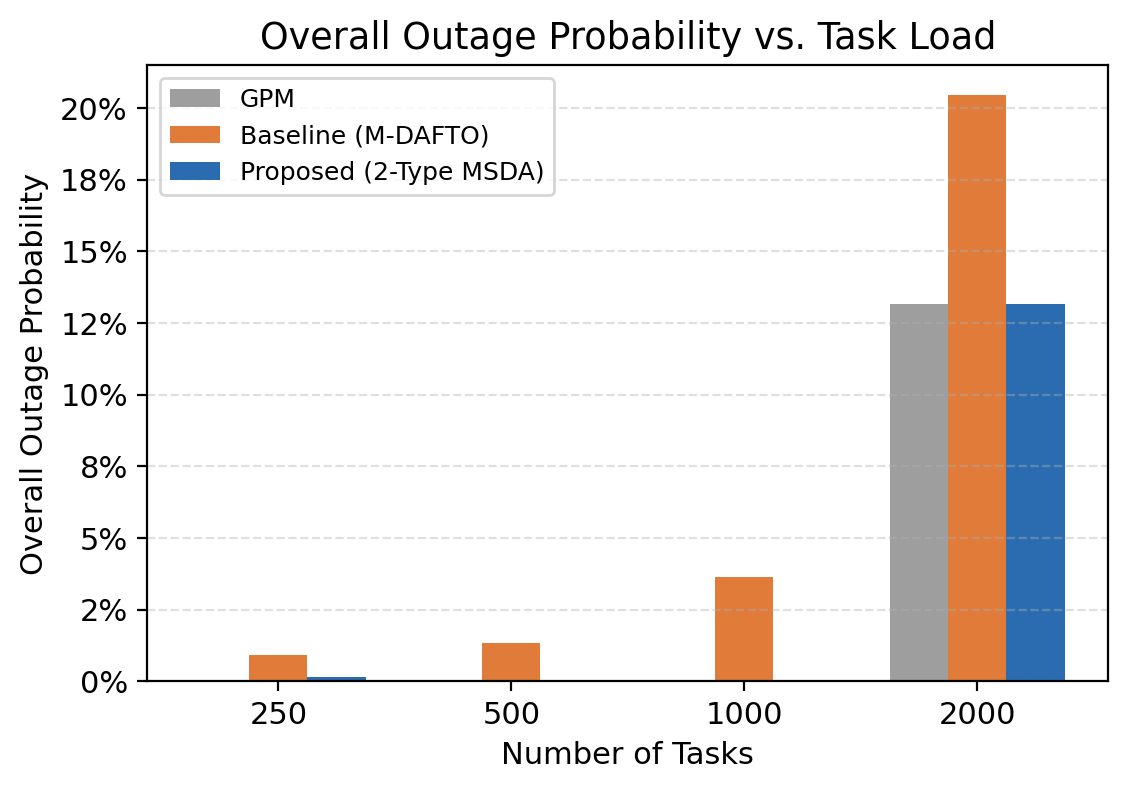
\includegraphics[width=0.75\textwidth]{Images/fig_overall_outage.png}
\caption{Overall outage probability comparison across four task scales.}
\label{fig:overall_outage}
\end{figure}

\begin{figure}[htbp]
\centering
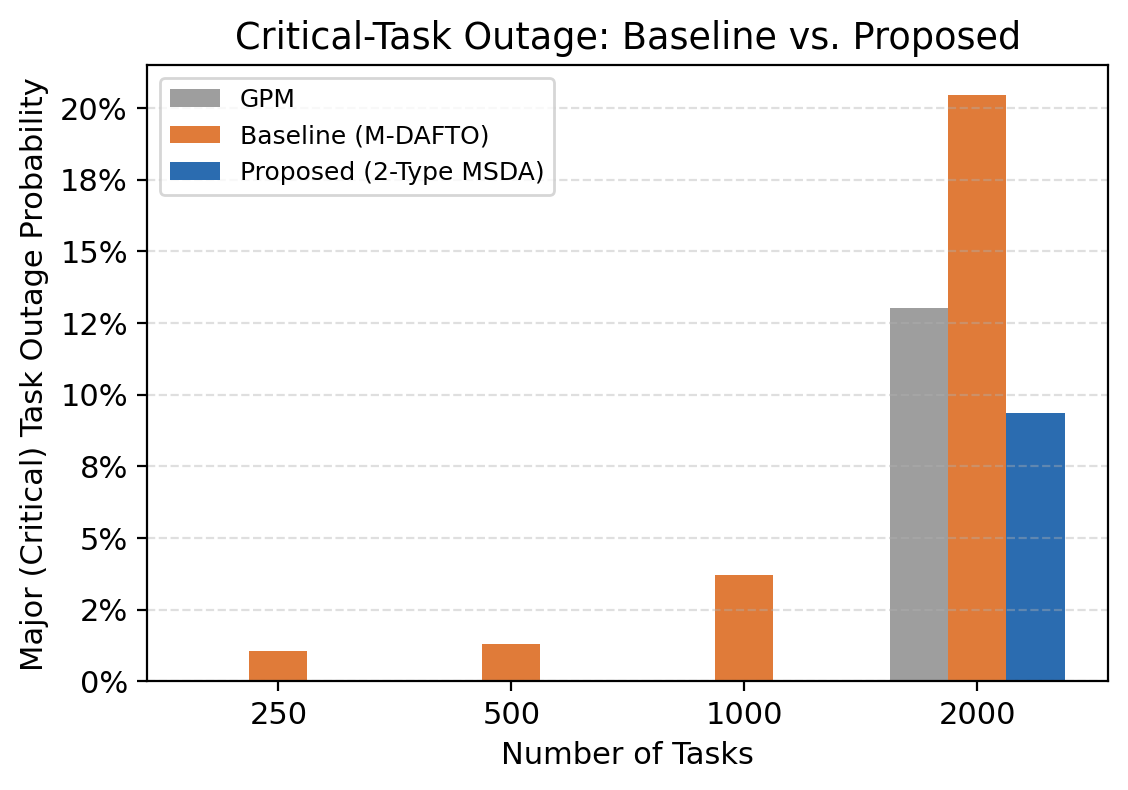
\includegraphics[width=0.75\textwidth]{Images/fig_major_outage.png}
\caption{Major task outage probability comparison across four task scales.}
\label{fig:major_outage}
\end{figure}

Table~\ref{tab:outage_reduction} summarises the outage reduction achieved by the proposed method relative to the baseline.

\begin{table}[htbp]
\centering
\begin{tabular}{|c|c|c|}
\hline
\textbf{Scale} & \textbf{Overall Outage Reduction} & \textbf{Major Outage Reduction} \\
\hline
250  & 82.6\% & $\sim$100\% \\
500  & 98.5\% & $\sim$100\% \\
1000 & 99.5\% & $\sim$100\% \\
2000 & 35.7\% & 54.3\% \\
\hline
\textbf{Average} & \textbf{$\sim$79\%} & \textbf{$\sim$89\%} \\
\hline
\end{tabular}
\caption{Outage reduction of the proposed method relative to the baseline M-DAFTO.}
\label{tab:outage_reduction}
\end{table}

The S-4 scenario (2000 tasks) represents extreme overload where total task demand exceeds the combined capacity of all fog nodes. Even in this saturated case, the proposed method still reduces Major outage by 54.3\%. The reduction is smaller than at lower scales because there are simply not enough fog node slots for all tasks, regardless of the matching algorithm used.

\section{Delay, Energy, and Satisfaction Trade-offs}

\subsection{Delay and Energy Comparison}

\begin{table}[htbp]
\centering
\begin{tabular}{|c|c|c|c|c|c|c|}
\hline
\textbf{Scale} & \multicolumn{2}{c|}{\textbf{Greedy Placement}} & \multicolumn{2}{c|}{\textbf{Baseline}} & \multicolumn{2}{c|}{\textbf{Proposed}} \\
\cline{2-7}
 & \textbf{AvgDelay} & \textbf{Energy} & \textbf{AvgDelay} & \textbf{Energy} & \textbf{AvgDelay} & \textbf{Energy} \\
\hline
250  & 20.66 & 5142.81 & 12.65 & 3102.92 & 12.87 & 3189.85 \\
500  & 20.43 & 10168.93 & 12.67 & 6186.92 & 12.83 & 6366.47 \\
1000 & 18.07 & 17976.69 & 13.36 & 12739.14 & 13.70 & 13604.51 \\
2000 & 16.17 & 28033.18 & 14.53 & 22967.31 & 16.22 & 28110.36 \\
\hline
\end{tabular}
\caption{Average delay (seconds) and total energy (Joules) across all algorithms.}
\label{tab:delay_energy}
\end{table}

The proposed method has slightly higher average delay than the baseline (e.g., 12.87 vs 12.65 at 250 tasks). This is because the 2-Type MSDA sacrifices delay-optimal placement to ensure Major tasks are assigned to fog nodes that satisfy the severity-aware quota constraints. In healthcare, this is an acceptable trade-off: a minor increase in processing delay is far preferable to a critical surgery going unassigned.

\subsection{Task and FN Satisfaction}

\begin{table}[htbp]
\centering
\begin{tabular}{|c|c|c|c|}
\hline
\textbf{Scale} & \textbf{Greedy Placement} & \textbf{Baseline (M-DAFTO)} & \textbf{Proposed System} \\
\hline
250  & 9.04\% & 71.14\% & 69.96\% \\
500  & 14.09\% & 68.26\% & 67.46\% \\
1000 & 21.72\% & 60.62\% & 59.31\% \\
2000 & 33.77\% & 40.27\% & 32.83\% \\
\hline
\end{tabular}
\caption{Task satisfaction (\%) across four task scales.}
\label{tab:task_satisfaction}
\end{table}

Task satisfaction is slightly lower for the proposed method (e.g., 69.96\% vs 71.14\% at 250 tasks) because the severity-aware matching sometimes assigns tasks to their second or third preferred fog node to ensure Major quotas are met. However, the difference is small (within 2 percentage points at most scales).

\begin{table}[htbp]
\centering
\begin{tabular}{|c|c|c|c|}
\hline
\textbf{Scale} & \textbf{Greedy Placement} & \textbf{Baseline (M-DAFTO)} & \textbf{Proposed System} \\
\hline
250  & 10.04\% & 10.54\% & 10.34\% \\
500  & 12.05\% & 19.50\% & 18.85\% \\
1000 & 25.00\% & 34.57\% & 35.25\% \\
2000 & 50.43\% & 50.22\% & \textbf{59.08\%} \\
\hline
\end{tabular}
\caption{FN satisfaction (\%) across four task scales.}
\label{tab:fn_satisfaction}
\end{table}

\begin{figure}[htbp]
\centering
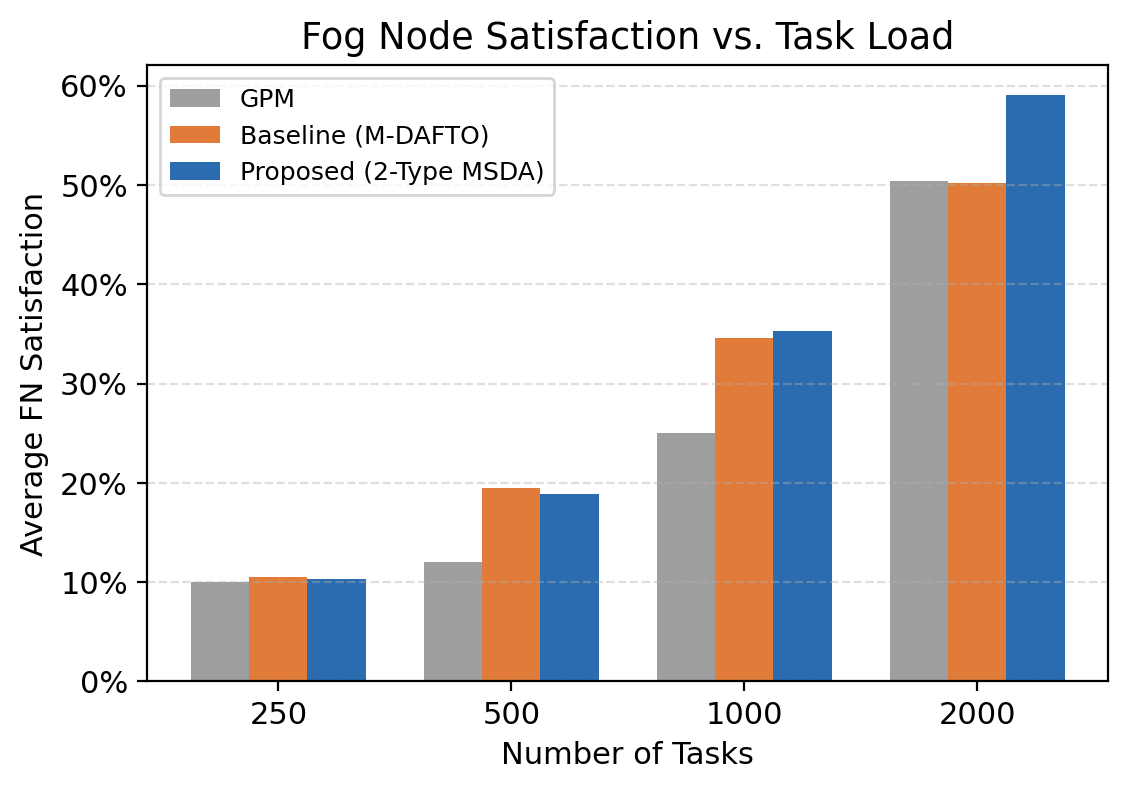
\includegraphics[width=0.75\textwidth]{Images/fig_fn_satisfaction.png}
\caption{FN satisfaction comparison across four task scales.}
\label{fig:fn_satisfaction}
\end{figure}

FN satisfaction improves under overload (59.08\% vs 50.22\% at 2000 tasks), showing that the 2-Type system distributes tasks more effectively by leveraging separate Major/Minor quota tracking.

\subsection{GPM Comparison}

GPM shows 0\% outage at 250--1000 tasks because it simply fills fog nodes greedily by capacity. However, its task satisfaction is extremely low (9--34\%) because it ignores preferences entirely. GPM fails at 2000 tasks (13.15\% outage) because it has no quota-based fairness mechanism. This confirms that greedy approaches, while simple, are unsuitable for healthcare IoT where both task satisfaction and critical-task protection matter.

\chapter{Conclusion}\label{chap:conclusion}
% --- CONCLUSION ---

\section{Summary of Contributions}

This project addressed the limitations of the M-DAFTO algorithm for healthcare IoT-fog task offloading by adapting the 2-Type Multi-Stage Deferred Acceptance (MSDA) algorithm from Oomori and Manabe \cite{oomori2026strategyproof} and combining it with several original extensions.

\subsection*{Adaptations of Prior Work}

\begin{enumerate}
\item \textbf{2-Type MSDA matching}: Adapted the 2-Type MSDA algorithm from \cite{oomori2026strategyproof} for IoT-fog task offloading, including the Modified DA with three simultaneous constraints and the final-stage three-case logic.

\item \textbf{Two-type task classification}: Applied the R-type/S-type framework from \cite{oomori2026strategyproof} by mapping Major/Minor healthcare task severity onto it, with separate quota constraints ($pr_c$, $qr_c$) per fog node ensuring critical tasks are never starved of resources.

\item \textbf{Separate preference lists}: Implemented separate fog-side rankings for all tasks, Major tasks only, and Minor tasks only, as structurally required by the 2-Type MSDA architecture \cite{oomori2026strategyproof}.
\end{enumerate}

\subsection*{Original Technical Additions}

\begin{enumerate}
\item \textbf{Energy as a metric}: Extended the urgency function to include energy consumption, computed from transmission, execution, and receiving power.

\item \textbf{Severity score}: Introduced a severity multiplier $\gamma$ (1.5 for Major, 1.0 for Minor) to the urgency formula, naturally prioritising critical tasks.

\item \textbf{Severity-weighted normalisation}: Designed a Min-Max normalisation applied to both delay and energy with severity-based weighting (0.5 for Minor, 1.0 for Major).

\item \textbf{4$\times$4 AHP}: Extended the AHP matrix from 2$\times$2 to 4$\times$4 with genuine consistency validation (CR $\leq$ 0.1).

\item \textbf{GPM baseline}: Implemented a Greedy Placement Method as an additional comparison point.
\end{enumerate}

On average across all tested scales, the adapted and extended method reduced overall outage by approximately 79\% and critical-task outage by approximately 89\% compared to the baseline. Under normal load (250--1000 tasks), the proposed algorithm achieves 0\% Major outage. These improvements come with acceptable trade-offs in delay and task satisfaction.

\section{Limitations}

Several limitations should be noted:
\begin{itemize}
\item \textbf{Batch processing}: The current system processes all tasks simultaneously in a batch. Real hospitals have continuous task arrivals that would require online/streaming processing.
\item \textbf{Synthetic data}: The evaluation uses randomly generated data rather than real healthcare workload traces. Testing with actual hospital data would validate practical viability.
\item \textbf{Narrow deadline range}: The deadline range of 15--22 seconds may not capture the full spectrum of healthcare urgency. Tasks requiring sub-second processing were not tested.
\item \textbf{Device-to-fog only}: The model supports only device-to-fog offloading. Fog-to-fog horizontal and fog-to-cloud vertical offloading are not considered.
\end{itemize}

\section{Future Work}

Several directions warrant future investigation:

\begin{itemize}
\item \textbf{Dynamic task arrival}: Extending the system to handle continuous, online task arrivals rather than batch processing, making it more realistic for hospital environments.

\item \textbf{Task migration}: Allowing tasks to be migrated between fog nodes when loads change dynamically, potentially improving performance under fluctuating conditions.

\item \textbf{Real-world workload traces}: Testing with actual healthcare workload traces from hospitals to validate the algorithm's practical viability.

\item \textbf{Heterogeneous deadlines}: Expanding the deadline range to include truly time-critical tasks (sub-second) and longer-horizon tasks, stressing the algorithm further.

\item \textbf{Fog-to-fog and fog-to-cloud offloading}: Adding horizontal (fog-to-fog) and vertical (fog-to-cloud) offloading to handle overflow scenarios more gracefully.

\item \textbf{Multi-tier severity}: Extending from 2 severity levels to 3 or more (e.g., Critical/Major/Minor/Routine) for finer-grained control.

\item \textbf{Machine learning weight generation}: Replacing the random AHP weight generation with learned weights from historical data, potentially improving performance.
\end{itemize}

%\clearpage
%\mbox{}
%\thispagestyle{empty}
%\newpage
%\addtocounter{page}{-1}
%\appendix
%%%..........................................................................................................................................
%\fancychapter{Appendix}\label{Sunil_Appendix}
%\chapter{Appendix}\label{Sunil_Appendix}
%  \include{Chapters/Appendix/Appendix}
%\clearpage
%%..........................................................................................................................................
%\fancychapter{Cepstral Analysis}
%\label{app:lpc}
%\include{chapters/Appendix/CFA}
%\clearpage
%%..........................................................................................................................................
%\fancychapter{Linear Prediction Coefficients Computation}
%\label{app:sine}
%\include{chapters/Appendix/Appendix_lpc_V2}
%\clearpage
%%..........................................................................................................................................
%\fancychapter{Composite Objective Quality Measures}
%\label{app:cqm}
%\include{Chapters/Appendix/Appendix_cqm_V1}
%\clearpage
%%..........................................................................................................................................
%\fancychapter{MFCC Feature Extraction}
%\label{app:mfcc}
%\include{Chapters/Appendix/Appendix_mfcc_V1}
%\clearpage
%%..........................................................................................................................................
%\fancychapter{Gaussian Mixture Models}
%\label{app:gmm}
%\include{Chapters/Appendix/Appendix_gmm_V1}
%\clearpage
%..........................................................................................................................................
%\doublespacing
%\normalsize
%\pdfbookmark{Publications}{Publications}
%\fancyhead[LE]{\bfseries\small{List of Publications}}
%\fancyhead[RO]{\bfseries\small{List of Publications}}
%\pdfbookmark[1]{List of Publications}{los}
%\addstarredchapter{List of Publications}
%\include{FrontPages/publ}
%\clearpage

%% LIST OF SYMBOLS
%\fancyhead[LE]{\bfseries\small{List of Symbols}}
%\fancyhead[RO]{\bfseries\small{List of Symbols}}
%\pdfbookmark[1]{List of Symbols}{los}
%\addstarredchapter{List of Symbols}
%\include{FrontPages/Symbols}
%\clearpage
%******************************************************************************************************************************************************************

%**************************************************BIBLIOGRAPHY********************************************************
% References Section
\fancyhead[LE]{\bfseries\small{Bibliography}}
\fancyhead[RO]{\bfseries\small{Bibliography}}
\pdfbookmark[1]{Bibliography}{los}
\addstarredchapter{Bibliography}   % Instead of Bibliography
\baselineskip 14pt   % Line spacing
\small
\bibliographystyle{IEEEtran}  % IEEE style

\bibliography{chapters/references/MyBibliography_2type_msda}
% \clearpage
%**************************************************PUBLICATIONS****************************************************************************************************************
\end{document}
